\chapter{Conception et Diagrammes UML}

\begin{objectivebox}
Ce chapitre présente la conception détaillée de l'application Housy Tunisia à travers différents diagrammes UML : cas d'utilisation, classes, séquences, architecture et pipeline de données.
\end{objectivebox}

\section{Diagramme de Cas d'Utilisation Général}

\subsection{Description}

Le diagramme de cas d'utilisation présente une vue d'ensemble des fonctionnalités principales de Housy Tunisia et des interactions entre les différents acteurs du système.

\subsection{Acteurs Identifiés}

\begin{itemize}
    \item \textbf{Administrateur :} Gestion complète du système
    \item \textbf{Chef de Projet :} Gestion des projets de construction
    \item \textbf{Estimateur :} Création et validation des devis
    \item \textbf{Client :} Consultation des projets et devis
    \item \textbf{Fournisseur :} Gestion du catalogue matériaux
    \item \textbf{Système Externe :} APIs tierces et services
\end{itemize}

\begin{figure}[h]
\centering
\begin{tikzpicture}[scale=0.8]
    % Acteurs
    \node[draw, ellipse] (admin) at (-8, 4) {Administrateur};
    \node[draw, ellipse] (chef) at (-8, 2) {Chef de Projet};
    \node[draw, ellipse] (estimateur) at (-8, 0) {Estimateur};
    \node[draw, ellipse] (client) at (-8, -2) {Client};
    \node[draw, ellipse] (fournisseur) at (-8, -4) {Fournisseur};
    \node[draw, ellipse] (systeme) at (8, 0) {Système Externe};
    
    % Système
    \draw[thick] (-2, -5) rectangle (6, 5);
    \node at (2, 4.5) {\textbf{Système Housy Tunisia}};
    
    % Cas d'utilisation principaux
    \node[draw, ellipse] (gestion_users) at (0, 3.5) {\parbox{2cm}{\centering Gérer\\Utilisateurs}};
    \node[draw, ellipse] (gestion_projets) at (2, 2.5) {\parbox{2cm}{\centering Gérer\\Projets}};
    \node[draw, ellipse] (estimation) at (4, 1.5) {\parbox{2cm}{\centering Créer\\Estimations}};
    \node[draw, ellipse] (planning) at (1, 1) {\parbox{2cm}{\centering Planifier\\Projets}};
    \node[draw, ellipse] (materiaaux) at (3, 0) {\parbox{2cm}{\centering Gérer\\Matériaux}};
    \node[draw, ellipse] (devis) at (5, -0.5) {\parbox{2cm}{\centering Générer\\Devis}};
    \node[draw, ellipse] (suivi) at (2, -1.5) {\parbox{2cm}{\centering Suivre\\Avancement}};
    \node[draw, ellipse] (reporting) at (4, -2.5) {\parbox{2cm}{\centering Générer\\Rapports}};
    \node[draw, ellipse] (consultation) at (1, -3) {\parbox{2cm}{\centering Consulter\\Projets}};
    \node[draw, ellipse] (authentification) at (0, -4) {\parbox{2cm}{\centering S'authentifier}};
    
    % Relations Administrateur
    \draw (admin) -- (gestion_users);
    \draw (admin) -- (gestion_projets);
    \draw (admin) -- (reporting);
    \draw (admin) -- (authentification);
    
    % Relations Chef de Projet
    \draw (chef) -- (gestion_projets);
    \draw (chef) -- (planning);
    \draw (chef) -- (suivi);
    \draw (chef) -- (reporting);
    \draw (chef) -- (authentification);
    
    % Relations Estimateur
    \draw (estimateur) -- (estimation);
    \draw (estimateur) -- (devis);
    \draw (estimateur) -- (materiaaux);
    \draw (estimateur) -- (authentification);
    
    % Relations Client
    \draw (client) -- (consultation);
    \draw (client) -- (authentification);
    
    % Relations Fournisseur
    \draw (fournisseur) -- (materiaaux);
    \draw (fournisseur) -- (authentification);
    
    % Relations Système Externe
    \draw (systeme) -- (estimation);
    \draw (systeme) -- (materiaaux);
    
\end{tikzpicture}
\caption{Diagramme de cas d'utilisation général - Housy Tunisia}
\end{figure}

\textbf{[CAPTURE À AJOUTER : Capture d'écran de l'interface principale montrant les fonctionnalités]}

\subsection{Cas d'Utilisation Détaillés}

\subsubsection{UC001 - Gérer les Projets de Construction}

\begin{itemize}
    \item \textbf{Acteur principal :} Chef de Projet
    \item \textbf{Préconditions :} Utilisateur authentifié avec droits appropriés
    \item \textbf{Scénario nominal :}
    \begin{enumerate}
        \item L'utilisateur accède au module de gestion des projets
        \item Il peut créer, modifier, supprimer ou consulter des projets
        \item Il définit les caractéristiques du projet (type, surface, localisation)
        \item Il assigne les ressources et définit le planning
        \item Le système sauvegarde et valide les informations
    \end{enumerate}
    \item \textbf{Postconditions :} Projet créé/modifié dans la base de données
\end{itemize}

\subsubsection{UC002 - Créer une Estimation}

\begin{itemize}
    \item \textbf{Acteur principal :} Estimateur
    \item \textbf{Préconditions :} Projet existant, base de prix à jour
    \item \textbf{Scénario nominal :}
    \begin{enumerate}
        \item L'estimateur sélectionne un projet
        \item Il renseigne les paramètres d'estimation
        \item Le système calcule automatiquement les coûts
        \item Il valide et ajuste si nécessaire
        \item Le système génère l'estimation finale
    \end{enumerate}
    \item \textbf{Postconditions :} Estimation sauvegardée et disponible
\end{itemize}

\section{Diagramme de Classes Global}

\subsection{Description}

Le diagramme de classes présente la structure orientée objet réelle de l'application Housy Tunisia, basée sur le schéma de base de données PostgreSQL avec Drizzle ORM.

\begin{figure}[h]
\centering
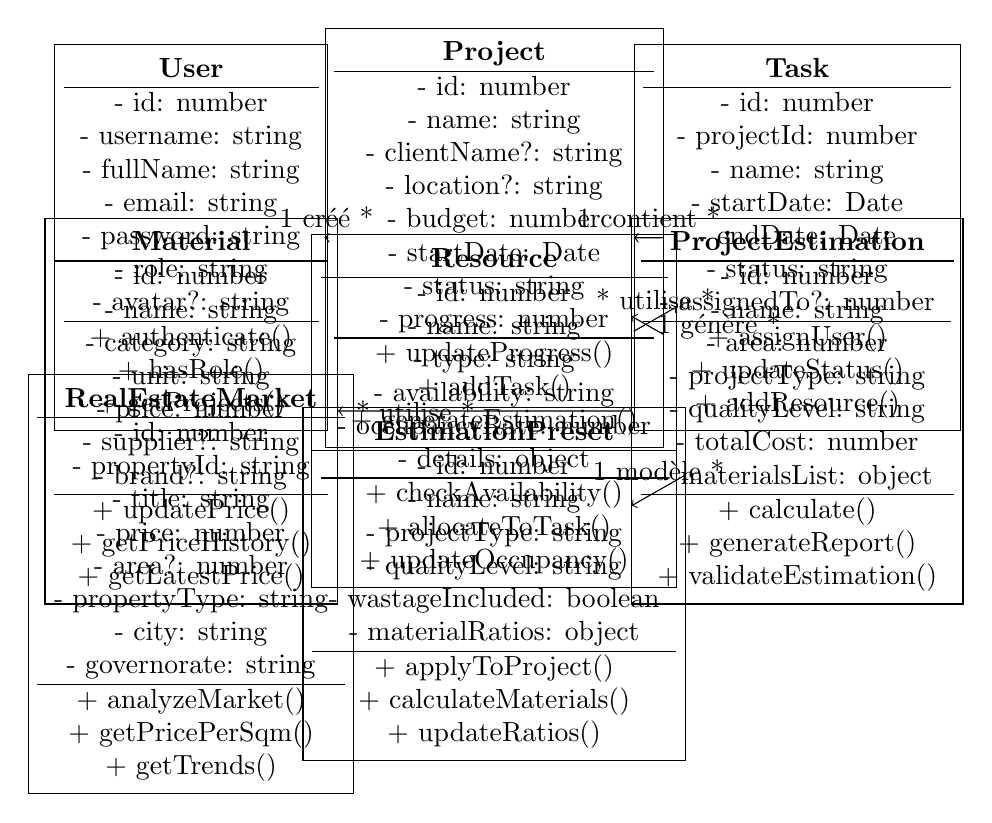
\begin{tikzpicture}[scale=0.55]
    % Classe User
    \node[draw, rectangle] (user) at (0, 10) {
        \begin{tabular}{c}
            \textbf{User} \\
            \hline
            - id: number \\
            - username: string \\
            - fullName: string \\
            - email: string \\
            - password: string \\
            - role: string \\
            - avatar?: string \\
            \hline
            + authenticate() \\
            + hasRole() \\
            + getProjects()
        \end{tabular}
    };
    
    % Classe Project
    \node[draw, rectangle] (project) at (7, 10) {
        \begin{tabular}{c}
            \textbf{Project} \\
            \hline
            - id: number \\
            - name: string \\
            - clientName?: string \\
            - location?: string \\
            - budget: number \\
            - startDate: Date \\
            - status: string \\
            - progress: number \\
            \hline
            + updateProgress() \\
            + addTask() \\
            + generateEstimation()
        \end{tabular}
    };
    
    % Classe Task
    \node[draw, rectangle] (task) at (14, 10) {
        \begin{tabular}{c}
            \textbf{Task} \\
            \hline
            - id: number \\
            - projectId: number \\
            - name: string \\
            - startDate: Date \\
            - endDate: Date \\
            - status: string \\
            - assignedTo?: number \\
            \hline
            + assignUser() \\
            + updateStatus() \\
            + addResource()
        \end{tabular}
    };
    
    % Classe Material
    \node[draw, rectangle] (material) at (0, 6) {
        \begin{tabular}{c}
            \textbf{Material} \\
            \hline
            - id: number \\
            - name: string \\
            - category: string \\
            - unit: string \\
            - price: number \\
            - supplier?: string \\
            - brand?: string \\
            \hline
            + updatePrice() \\
            + getPriceHistory() \\
            + getLatestPrice()
        \end{tabular}
    };
    
    % Classe Resource
    \node[draw, rectangle] (resource) at (7, 6) {
        \begin{tabular}{c}
            \textbf{Resource} \\
            \hline
            - id: number \\
            - name: string \\
            - type: string \\
            - availability: string \\
            - occupancyRate: number \\
            - details: object \\
            \hline
            + checkAvailability() \\
            + allocateToTask() \\
            + updateOccupancy()
        \end{tabular}
    };
    
    % Classe ProjectEstimation
    \node[draw, rectangle] (estimation) at (14, 6) {
        \begin{tabular}{c}
            \textbf{ProjectEstimation} \\
            \hline
            - id: number \\
            - name: string \\
            - area: number \\
            - projectType: string \\
            - qualityLevel: string \\
            - totalCost: number \\
            - materialsList: object \\
            \hline
            + calculate() \\
            + generateReport() \\
            + validateEstimation()
        \end{tabular}
    };
    
    % Classe RealEstateMarket
    \node[draw, rectangle] (market) at (0, 2) {
        \begin{tabular}{c}
            \textbf{RealEstateMarket} \\
            \hline
            - id: number \\
            - propertyId: string \\
            - title: string \\
            - price: number \\
            - area?: number \\
            - propertyType: string \\
            - city: string \\
            - governorate: string \\
            \hline
            + analyzeMarket() \\
            + getPricePerSqm() \\
            + getTrends()
        \end{tabular}
    };
    
    % Classe EstimationPreset
    \node[draw, rectangle] (preset) at (7, 2) {
        \begin{tabular}{c}
            \textbf{EstimationPreset} \\
            \hline
            - id: number \\
            - name: string \\
            - projectType: string \\
            - qualityLevel: string \\
            - wastageIncluded: boolean \\
            - materialRatios: object \\
            \hline
            + applyToProject() \\
            + calculateMaterials() \\
            + updateRatios()
        \end{tabular}
    };
    
    % Relations
    \draw[->] (user) -- (project) node[midway, above] {1 créé *};
    \draw[->] (project) -- (task) node[midway, above] {1 contient *};
    \draw[->] (project) -- (estimation) node[midway, right] {1 génère *};
    \draw[->] (task) -- (resource) node[midway, above] {* utilise *};
    \draw[->] (estimation) -- (material) node[midway, left] {* utilise *};
    \draw[->] (preset) -- (estimation) node[midway, above] {1 modèle *};
    
\end{tikzpicture}
\caption{Diagramme de classes basé sur le schéma Drizzle ORM réel}
\end{figure}
        \begin{tabular}{c}
            \textbf{Project} \\
            \hline
            - id: number \\
            - name: string \\
            - type: ProjectType \\
            - surface: number \\
            - status: ProjectStatus \\
            - clientId: number \\
            - managerId: number \\
            \hline
            + calculateCost() \\
            + updateStatus() \\
            + generateReport()
        \end{tabular}
    };
    
    % Classe Estimation
    \node[draw, rectangle] (estimation) at (12, 8) {
        \begin{tabular}{c}
            \textbf{Estimation} \\
            \hline
            - id: number \\
            - projectId: number \\
            - totalCost: number \\
            - materialCost: number \\
            - laborCost: number \\
            - currency: string \\
            \hline
            + calculate() \\
            + export() \\
            + validate()
        \end{tabular}
    };
    
    % Classe Material
    \node[draw, rectangle] (material) at (0, 4) {
        \begin{tabular}{c}
            \textbf{Material} \\
            \hline
            - id: number \\
            - name: string \\
            - category: string \\
            - unit: string \\
            - pricePerUnit: number \\
            - supplierId: number \\
            \hline
            + updatePrice() \\
            + checkStock() \\
            + getHistory()
        \end{tabular}
    };
    
    % Classe Supplier
    \node[draw, rectangle] (supplier) at (6, 4) {
        \begin{tabular}{c}
            \textbf{Supplier} \\
            \hline
            - id: number \\
            - name: string \\
            - contact: string \\
            - address: string \\
            - phone: string \\
            - email: string \\
            \hline
            + addMaterial() \\
            + updateCatalog() \\
            + generateOrder()
        \end{tabular}
    };
    
    % Classe Task
    \node[draw, rectangle] (task) at (12, 4) {
        \begin{tabular}{c}
            \textbf{Task} \\
            \hline
            - id: number \\
            - projectId: number \\
            - name: string \\
            - description: string \\
            - status: TaskStatus \\
            - assigneeId: number \\
            \hline
            + assign() \\
            + complete() \\
            + updateProgress()
        \end{tabular}
    };
    
    % Classe Client
    \node[draw, rectangle] (client) at (0, 0) {
        \begin{tabular}{c}
            \textbf{Client} \\
            \hline
            - id: number \\
            - name: string \\
            - type: ClientType \\
            - contact: string \\
            - address: string \\
            \hline
            + createProject() \\
            + approveEstimation() \\
            + makePayment()
        \end{tabular}
    };
    
    % Relations
    \draw[->] (user) -- (project) node[midway, above] {manages};
    \draw[->] (project) -- (estimation) node[midway, above] {has};
    \draw[->] (project) -- (task) node[midway, above] {contains};
    \draw[->] (material) -- (supplier) node[midway, above] {supplied by};
    \draw[->] (client) -- (project) node[midway, left] {owns};
    \draw[->] (estimation) -- (material) node[midway, left] {uses};
    
\end{tikzpicture}
\caption{Diagramme de classes global - Architecture principale}
\end{figure}

\subsection{Description des Classes Principales}

\subsubsection{Classe User}
- Représente tous les utilisateurs du système
- Gère l'authentification et les permissions
- Support des rôles : Admin, Manager, Estimator, Client

\subsubsection{Classe Project}
- Entité centrale représentant un projet de construction
- Contient toutes les informations du projet
- Méthodes de calcul et de gestion du cycle de vie

\subsubsection{Classe Estimation}
- Représente une estimation de coût
- Calculs automatisés basés sur les matériaux et main-d'œuvre
- Export en différents formats

\textbf{[CAPTURE À AJOUTER : Capture de l'interface de gestion des classes dans l'IDE]}

\section{Architecture de l'Application}

\subsection{Architecture Technique Globale}

\begin{figure}[h]
\centering
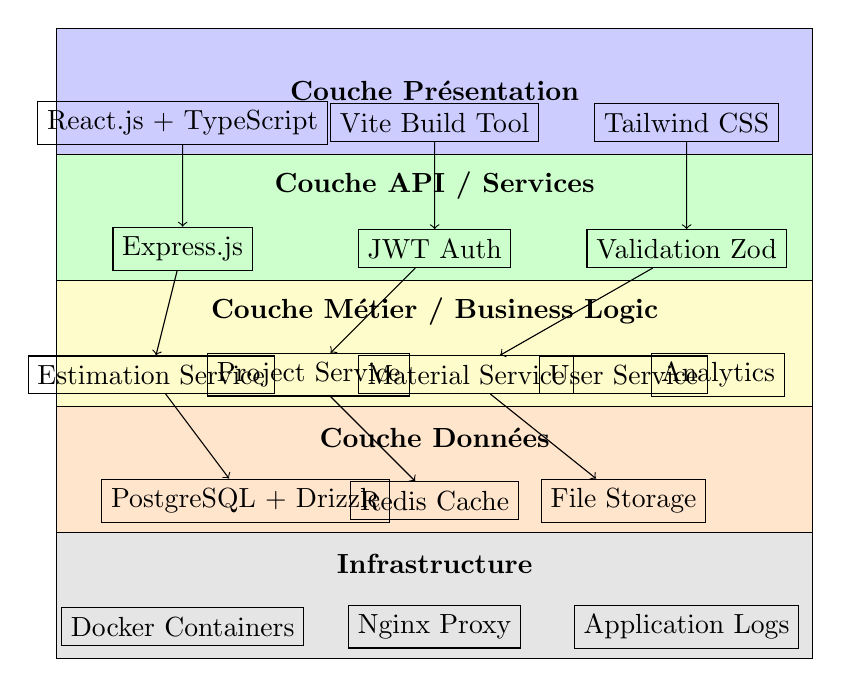
\begin{tikzpicture}[scale=0.8]
    % Couche Présentation
    \draw[fill=blue!20] (0, 8) rectangle (12, 10);
    \node at (6, 9) {\textbf{Couche Présentation}};
    
    \node[draw, rectangle] (react) at (2, 8.5) {React.js + TypeScript};
    \node[draw, rectangle] (vite) at (6, 8.5) {Vite Build Tool};
    \node[draw, rectangle] (tailwind) at (10, 8.5) {Tailwind CSS};
    
    % Couche API
    \draw[fill=green!20] (0, 6) rectangle (12, 8);
    \node at (6, 7.5) {\textbf{Couche API / Services}};
    
    \node[draw, rectangle] (express) at (2, 6.5) {Express.js};
    \node[draw, rectangle] (auth) at (6, 6.5) {JWT Auth};
    \node[draw, rectangle] (validation) at (10, 6.5) {Validation Zod};
    
    % Couche Métier
    \draw[fill=yellow!20] (0, 4) rectangle (12, 6);
    \node at (6, 5.5) {\textbf{Couche Métier / Business Logic}};
    
    \node[draw, rectangle] (estimation) at (1.5, 4.5) {Estimation Service};
    \node[draw, rectangle] (project) at (4, 4.5) {Project Service};
    \node[draw, rectangle] (material) at (6.5, 4.5) {Material Service};
    \node[draw, rectangle] (user) at (9, 4.5) {User Service};
    \node[draw, rectangle] (analytics) at (10.5, 4.5) {Analytics};
    
    % Couche Données
    \draw[fill=orange!20] (0, 2) rectangle (12, 4);
    \node at (6, 3.5) {\textbf{Couche Données}};
    
    \node[draw, rectangle] (postgres) at (3, 2.5) {PostgreSQL + Drizzle};
    \node[draw, rectangle] (redis) at (6, 2.5) {Redis Cache};
    \node[draw, rectangle] (files) at (9, 2.5) {File Storage};
    
    % Infrastructure
    \draw[fill=gray!20] (0, 0) rectangle (12, 2);
    \node at (6, 1.5) {\textbf{Infrastructure}};
    
    \node[draw, rectangle] (docker) at (2, 0.5) {Docker Containers};
    \node[draw, rectangle] (nginx) at (6, 0.5) {Nginx Proxy};
    \node[draw, rectangle] (logs) at (10, 0.5) {Application Logs};
    
    % Flèches
    \draw[->] (react) -- (express);
    \draw[->] (vite) -- (auth);
    \draw[->] (tailwind) -- (validation);
    
    \draw[->] (express) -- (estimation);
    \draw[->] (auth) -- (project);
    \draw[->] (validation) -- (material);
    
    \draw[->] (estimation) -- (postgres);
    \draw[->] (project) -- (redis);
    \draw[->] (material) -- (files);
    
\end{tikzpicture}
\caption{Architecture technique réelle en couches}
\end{figure}

\subsection{Explication de l'Architecture}

\subsubsection{Couche Présentation}
- \textbf{React.js + TypeScript :} Interface utilisateur moderne et typée avec ShadCN/UI
- \textbf{Vite :} Build tool rapide pour le développement et la production
- \textbf{Tailwind CSS :} Framework CSS utility-first pour le styling

\subsubsection{Couche API}
- \textbf{Express.js :} Framework web Node.js avec middleware de sécurité
- \textbf{JWT Auth :} Authentification basée sur tokens avec Passport.js
- \textbf{Validation Zod :} Validation des données d'entrée avec schémas TypeScript

\subsubsection{Couche Métier}
- Services encapsulant la logique business
- Module d'estimation avec intégration IA (OpenAI, Anthropic)
- Analytics internes pour le suivi des métriques
- Séparation claire des responsabilités

\subsubsection{Couche Données}
- \textbf{PostgreSQL + Drizzle :} Base de données relationnelle avec ORM typé
- \textbf{Redis :} Cache pour optimiser les performances des sessions
- \textbf{File Storage :} Stockage des documents et images uploadés

\subsubsection{Infrastructure}
- \textbf{Docker Containers :} Containerisation pour la portabilité
- \textbf{Nginx Proxy :} Reverse proxy et load balancer
- \textbf{Application Logs :} Système de logs avec Winston

\textbf{[CAPTURE À AJOUTER : Vue d'ensemble de l'architecture dans un outil de diagramme]}

\section{Architecture du Pipeline de Données}

\subsection{Pipeline d'Estimation}

\begin{figure}[h]
\centering
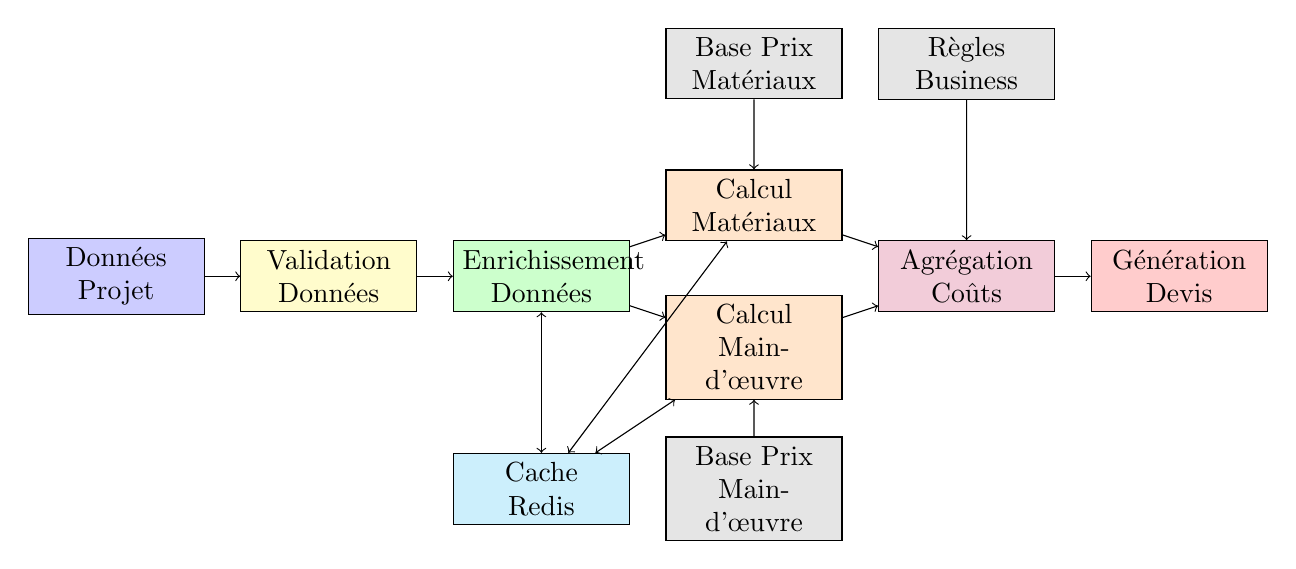
\begin{tikzpicture}[scale=0.9]
    % Début du pipeline
    \node[draw, rectangle, fill=blue!20] (input) at (0, 6) {\parbox{2cm}{\centering Données\\Projet}};
    
    % Validation
    \node[draw, rectangle, fill=yellow!20] (validation) at (3, 6) {\parbox{2cm}{\centering Validation\\Données}};
    
    % Enrichissement
    \node[draw, rectangle, fill=green!20] (enrichment) at (6, 6) {\parbox{2cm}{\centering Enrichissement\\Données}};
    
    % Calcul matériaux
    \node[draw, rectangle, fill=orange!20] (materials) at (9, 7) {\parbox{2cm}{\centering Calcul\\Matériaux}};
    
    % Calcul main-d'œuvre
    \node[draw, rectangle, fill=orange!20] (labor) at (9, 5) {\parbox{2cm}{\centering Calcul\\Main-d'œuvre}};
    
    % Agrégation
    \node[draw, rectangle, fill=purple!20] (aggregation) at (12, 6) {\parbox{2cm}{\centering Agrégation\\Coûts}};
    
    % Génération rapport
    \node[draw, rectangle, fill=red!20] (report) at (15, 6) {\parbox{2cm}{\centering Génération\\Devis}};
    
    % Sources de données
    \node[draw, rectangle, fill=gray!20] (db_materials) at (9, 9) {\parbox{2cm}{\centering Base Prix\\Matériaux}};
    \node[draw, rectangle, fill=gray!20] (db_labor) at (9, 3) {\parbox{2cm}{\centering Base Prix\\Main-d'œuvre}};
    \node[draw, rectangle, fill=gray!20] (rules) at (12, 9) {\parbox{2cm}{\centering Règles\\Business}};
    
    % Cache
    \node[draw, rectangle, fill=cyan!20] (cache) at (6, 3) {\parbox{2cm}{\centering Cache\\Redis}};
    
    % Flèches principales
    \draw[->] (input) -- (validation);
    \draw[->] (validation) -- (enrichment);
    \draw[->] (enrichment) -- (materials);
    \draw[->] (enrichment) -- (labor);
    \draw[->] (materials) -- (aggregation);
    \draw[->] (labor) -- (aggregation);
    \draw[->] (aggregation) -- (report);
    
    % Flèches sources de données
    \draw[->] (db_materials) -- (materials);
    \draw[->] (db_labor) -- (labor);
    \draw[->] (rules) -- (aggregation);
    
    % Cache
    \draw[<->] (enrichment) -- (cache);
    \draw[<->] (materials) -- (cache);
    \draw[<->] (labor) -- (cache);
    
\end{tikzpicture}
\caption{Pipeline de traitement des estimations}
\end{figure}

\subsection{Description du Pipeline}

\subsubsection{Étapes du Pipeline}

\begin{enumerate}
    \item \textbf{Données Projet :} Saisie des caractéristiques du projet
    \item \textbf{Validation :} Contrôle de cohérence et complétude
    \item \textbf{Enrichissement :} Ajout de données contextuelles
    \item \textbf{Calculs Parallèles :} Matériaux et main-d'œuvre en parallèle
    \item \textbf{Agrégation :} Combinaison des coûts avec règles business
    \item \textbf{Génération :} Production du devis final
\end{enumerate}

\subsubsection{Sources de Données}
- Base de prix des matériaux tunisiens
- Tarifs main-d'œuvre par région
- Règles business et coefficients
- Cache Redis pour l'optimisation

\textbf{[CAPTURE À AJOUTER : Interface de monitoring du pipeline en temps réel]}

\section{Diagrammes de Séquence}

\subsection{Séquence : Création d'un Projet}

\begin{figure}[h]
\centering
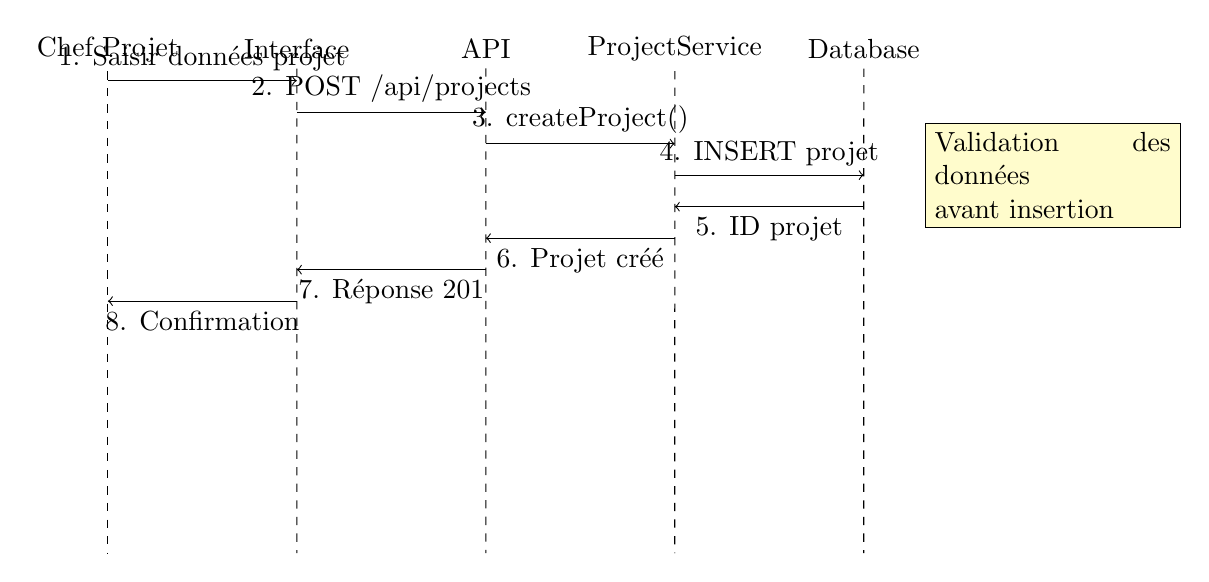
\begin{tikzpicture}[scale=0.8]
    % Acteurs
    \node (user) at (0, 8) {Chef Projet};
    \node (ui) at (3, 8) {Interface};
    \node (api) at (6, 8) {API};
    \node (service) at (9, 8) {ProjectService};
    \node (db) at (12, 8) {Database};
    
    % Lignes de vie
    \draw[dashed] (user) -- (0, 0);
    \draw[dashed] (ui) -- (3, 0);
    \draw[dashed] (api) -- (6, 0);
    \draw[dashed] (service) -- (9, 0);
    \draw[dashed] (db) -- (12, 0);
    
    % Messages
    \draw[->] (0, 7.5) -- (3, 7.5) node[midway, above] {1. Saisir données projet};
    \draw[->] (3, 7) -- (6, 7) node[midway, above] {2. POST /api/projects};
    \draw[->] (6, 6.5) -- (9, 6.5) node[midway, above] {3. createProject()};
    \draw[->] (9, 6) -- (12, 6) node[midway, above] {4. INSERT projet};
    \draw[<-] (9, 5.5) -- (12, 5.5) node[midway, below] {5. ID projet};
    \draw[<-] (6, 5) -- (9, 5) node[midway, below] {6. Projet créé};
    \draw[<-] (3, 4.5) -- (6, 4.5) node[midway, below] {7. Réponse 201};
    \draw[<-] (0, 4) -- (3, 4) node[midway, below] {8. Confirmation};
    
    % Notes
    \node[draw, rectangle, fill=yellow!20] at (15, 6) {\parbox{3cm}{Validation des données\\avant insertion}};
    
\end{tikzpicture}
\caption{Diagramme de séquence - Création d'un projet}
\end{figure}

\subsection{Séquence : Génération d'Estimation}

\begin{figure}[h]
\centering
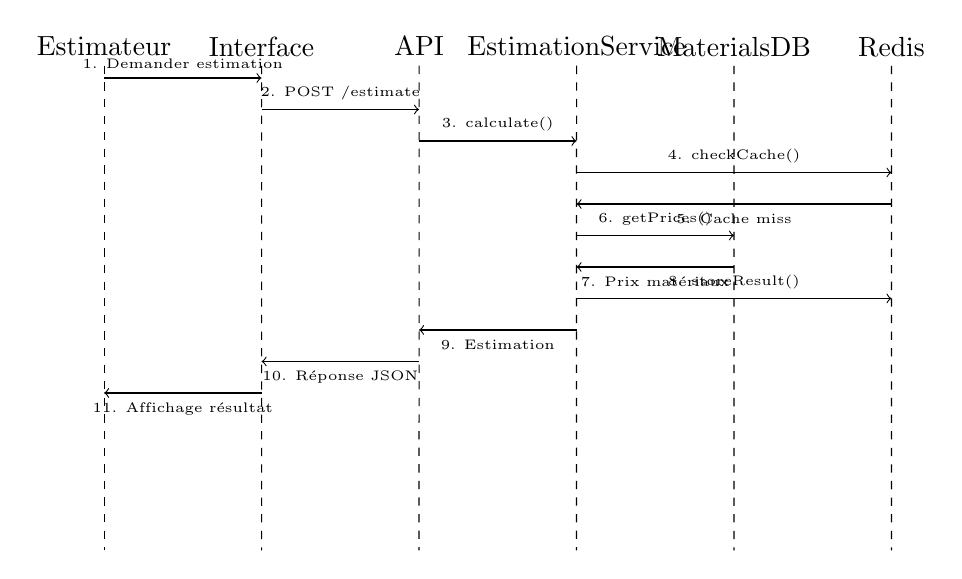
\begin{tikzpicture}[scale=0.8]
    % Acteurs
    \node (estimator) at (0, 8) {Estimateur};
    \node (ui) at (2.5, 8) {Interface};
    \node (api) at (5, 8) {API};
    \node (service) at (7.5, 8) {EstimationService};
    \node (materials) at (10, 8) {MaterialsDB};
    \node (cache) at (12.5, 8) {Redis};
    
    % Lignes de vie
    \draw[dashed] (estimator) -- (0, 0);
    \draw[dashed] (ui) -- (2.5, 0);
    \draw[dashed] (api) -- (5, 0);
    \draw[dashed] (service) -- (7.5, 0);
    \draw[dashed] (materials) -- (10, 0);
    \draw[dashed] (cache) -- (12.5, 0);
    
    % Messages
    \draw[->] (0, 7.5) -- (2.5, 7.5) node[midway, above] {\tiny 1. Demander estimation};
    \draw[->] (2.5, 7) -- (5, 7) node[midway, above] {\tiny 2. POST /estimate};
    \draw[->] (5, 6.5) -- (7.5, 6.5) node[midway, above] {\tiny 3. calculate()};
    
    % Vérification cache
    \draw[->] (7.5, 6) -- (12.5, 6) node[midway, above] {\tiny 4. checkCache()};
    \draw[<-] (7.5, 5.5) -- (12.5, 5.5) node[midway, below] {\tiny 5. Cache miss};
    
    % Récupération prix
    \draw[->] (7.5, 5) -- (10, 5) node[midway, above] {\tiny 6. getPrices()};
    \draw[<-] (7.5, 4.5) -- (10, 4.5) node[midway, below] {\tiny 7. Prix matériaux};
    
    % Calcul et cache
    \draw[->] (7.5, 4) -- (12.5, 4) node[midway, above] {\tiny 8. storeResult()};
    \draw[<-] (5, 3.5) -- (7.5, 3.5) node[midway, below] {\tiny 9. Estimation};
    \draw[<-] (2.5, 3) -- (5, 3) node[midway, below] {\tiny 10. Réponse JSON};
    \draw[<-] (0, 2.5) -- (2.5, 2.5) node[midway, below] {\tiny 11. Affichage résultat};
    
\end{tikzpicture}
\caption{Diagramme de séquence - Génération d'estimation}
\end{figure}

\subsection{Séquence : Authentification Utilisateur}

\begin{figure}[h]
\centering
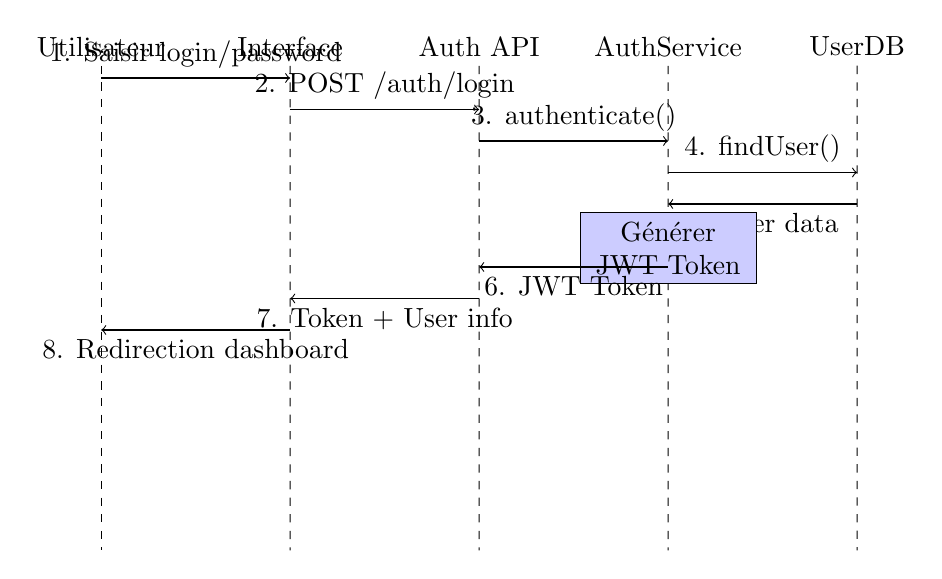
\begin{tikzpicture}[scale=0.8]
    % Acteurs
    \node (user) at (0, 8) {Utilisateur};
    \node (ui) at (3, 8) {Interface};
    \node (api) at (6, 8) {Auth API};
    \node (auth) at (9, 8) {AuthService};
    \node (db) at (12, 8) {UserDB};
    
    % Lignes de vie
    \draw[dashed] (user) -- (0, 0);
    \draw[dashed] (ui) -- (3, 0);
    \draw[dashed] (api) -- (6, 0);
    \draw[dashed] (auth) -- (9, 0);
    \draw[dashed] (db) -- (12, 0);
    
    % Messages
    \draw[->] (0, 7.5) -- (3, 7.5) node[midway, above] {1. Saisir login/password};
    \draw[->] (3, 7) -- (6, 7) node[midway, above] {2. POST /auth/login};
    \draw[->] (6, 6.5) -- (9, 6.5) node[midway, above] {3. authenticate()};
    \draw[->] (9, 6) -- (12, 6) node[midway, above] {4. findUser()};
    \draw[<-] (9, 5.5) -- (12, 5.5) node[midway, below] {5. User data};
    
    % Génération token
    \node[draw, rectangle, fill=blue!20] at (9, 4.8) {\parbox{2cm}{\centering Générer\\JWT Token}};
    
    \draw[<-] (6, 4.5) -- (9, 4.5) node[midway, below] {6. JWT Token};
    \draw[<-] (3, 4) -- (6, 4) node[midway, below] {7. Token + User info};
    \draw[<-] (0, 3.5) -- (3, 3.5) node[midway, below] {8. Redirection dashboard};
    
\end{tikzpicture}
\caption{Diagramme de séquence - Authentification}
\end{figure}

\section{Placement des Diagrammes dans le Rapport}

\subsection{Recommandations de Placement}

\begin{table}[h]
\centering
\begin{tabular}{|l|l|l|}
\hline
\textbf{Diagramme} & \textbf{Chapitre Recommandé} & \textbf{Section} \\
\hline
Cas d'utilisation général & Chapitre 3 - Business Understanding & Analyse des besoins \\
\hline
Diagramme de classes & Chapitre 5 - Modélisation & Architecture technique \\
\hline
Architecture application & Chapitre 5 - Modélisation & Conception système \\
\hline
Pipeline de données & Chapitre 4 - Data Preparation & Processus de traitement \\
\hline
Séquences principales & Chapitre 5 - Modélisation & Interactions système \\
\hline
\end{tabular}
\caption{Placement recommandé des diagrammes}
\end{table}

\subsection{Captures d'Écran Complémentaires}

Pour chaque diagramme, prévoir les captures suivantes :

\begin{itemize}
    \item \textbf{Interface utilisateur :} Capture montrant les fonctionnalités en action
    \item \textbf{Code source :} Extraits de code correspondant aux diagrammes
    \item \textbf{Monitoring :} Dashboards montrant le système en fonctionnement
    \item \textbf{Tests :} Résultats des tests validant les fonctionnalités
\end{itemize}

\textbf{[CAPTURE À AJOUTER : Ensemble de captures montrant les différents aspects du système]}

\begin{resultbox}
Ces diagrammes UML fournissent une vue complète de la conception de Housy Tunisia, depuis les besoins utilisateurs jusqu'à l'architecture technique détaillée. Ils constituent la documentation de référence pour le développement et la maintenance de l'application.
\end{resultbox}
